\subsection{Оценка точности моделей ядерных масс}
Описанные в настоящем разделе ядерные модели использовались нами для расчета скоростей реакций нейтронного захвата, участвующих в астрофизическом $r$-процессе. Выбор именно этих моделей обусловлен тем, что каждая из них реализует отдельный подход к предсказанию масс экзотических ядер. Будет интересно посмотреть, как различные методы расчета ядерных масс влияют на результаты моделирования $r$-процесса.

\begin{figure}
  \centering
  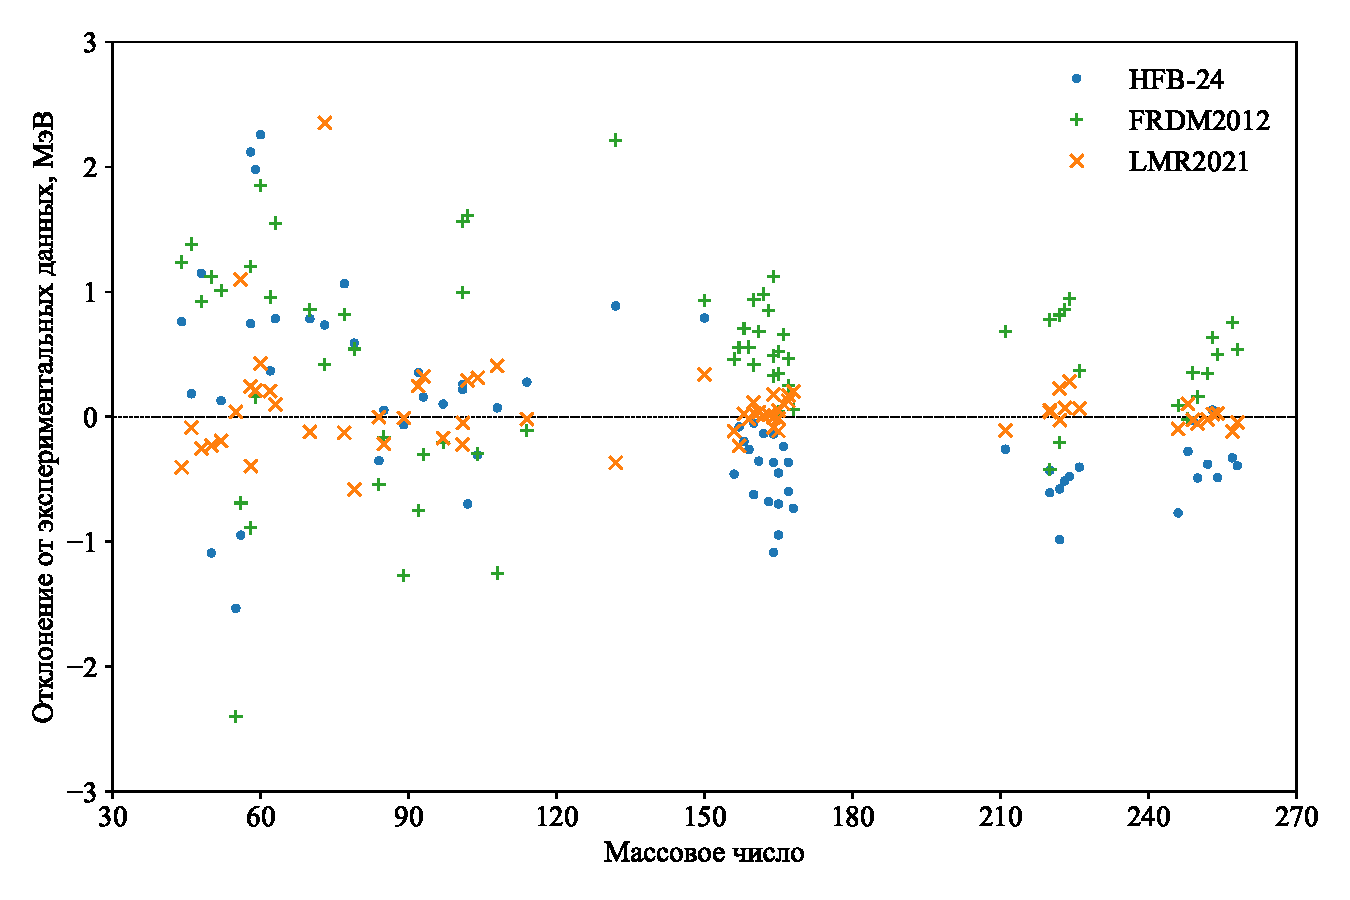
\includegraphics[width=0.9\textwidth]{../pics/deviations.pdf}
  \caption{Разница теоретических энергий связи из таблиц FRDM2012~\cite{moller2016}, HFB-24~\cite{goriely2013} и специальной версии LMR2021~\cite{vladimirova2022} (см.пояснение в тексте) и экспериментальных значений из базы данных AME2020~\cite{huang2021}.}
  \label{fig:deviations}
\end{figure}

Для нас наиболее интересны предсказания масс изотопов с большим избытком нейтронов, которые не могут быть получены в лабораторных условиях. Оценить точность теоретических моделей в этой области $NZ$-диаграммы не представляется возможным в силу отсутствия экспериментальных данных. Тем не менее можно проанализировать точность предсказания моделей вблизи долины стабильности. Для этого мы исследовали отклонения теоретических энергий связи от экспериментальных значений из базы данных AME2020 для ряда ядер. При этом в качестве таблицы LMR2021 использовалась специальная версия, рассчитанная описанным выше методом, но на основе базы данных AME2016, а не более новой AME2020. Использование именно этой версии таблицы обусловлено тем, что в массовую таблицу LMR2021 исходные экспериментальные данные входят без изменений, поэтому сравнивать стандартную версию таблицы с AME2020 было бы некорректно.

На рис.~\ref{fig:deviations} представлены результаты этого сравнения. Среднеквадратичные отклонения составляют $0.73$~МэВ для HFB-24, $0.89$~МэВ для FRDM2012 и $0.37$~МэВ для специальной версии LMR2021. Как видно, для новых экспериментальных данных, появившихся в последней версии AME2020
предсказания всех трех моделей имеют значительные флуктуации в области легких ядер. Для массовых чисел $A > 120$ модель FRDM2012 заметно завышает, а HFB-24 занижает величину энергии связи. Метод локальных массовых соотношений LMR2021 при этом обладает наивысшей точностью. Это может быть связано с тем, что методом LMR2021 коллективные и микроскопические эффекты учитываются неявно за счет исходных экспериментальных данных, не делается никаких сильных предположений о структуре и физике ядер. 

Однако точность предсказаний на малом удалении от долины стабильности не гарантирует ее сохранение в области сверхнейтроноизбыточных изотопов, где в основном протекает $r$-процесс. Безусловно для развития понимания астрофизического $r$-процесса и нуклеосинтеза в целом необходимо совершенствовать наши представления о физике нейтроноизбыточных ядер.

